\documentclass{beamer}
\usepackage[utf8]{inputenc}
\usepackage{helvet}
\usepackage{caption}
\usepackage{xcolor}
\renewcommand{\familydefault}{\sfdefault}

% Define colors
\definecolor{Blue}{RGB}{0, 40, 165} % UZH Blue
\definecolor{LightBlue}{RGB}{48, 98, 255} % UZH Light Blue
\definecolor{Green}{RGB}{164, 210, 51} % UZH Green



% Apply colors
\setbeamercolor{itemize item}{fg=LightBlue}
\setbeamercolor{itemize subitem}{fg=LightBlue}
\setbeamercolor{itemize subsubitem}{fg=LightBlue}
\setbeamercolor{author in head/foot}{bg=Blue, fg=white}
\setbeamercolor{title in head/foot}{bg=Blue, fg=white}
\setbeamercolor{title}{fg=Blue}
\setbeamercolor{section in toc}{fg=black}
\setbeamercolor{frametitle}{fg=Blue}


% Footline settings
\setbeamertemplate{footline}{%
  \leavevmode%
  \hbox{%
  \begin{beamercolorbox}[wd=\paperwidth,ht=2.25ex,dp=1ex]{author in head/foot}%
    \usebeamerfont{author in head/foot}%
    \makebox[.3333\paperwidth][l]{\hspace{0.3cm}\myclass\hskip.5cm}%
    \makebox[.3333\paperwidth][c]{\shorttitle}%
    \makebox[.3333\paperwidth][r]{\hskip.5cm\insertframenumber/\inserttotalframenumber\hspace{0.3cm}}%
  \end{beamercolorbox}}%
  \vskip0pt%
}

\newcommand{\myclass}{Digital Tools in Finance HS24}
\newcommand{\shorttitle}{Gender Pay Gap in Switzerland}

% Table of Contents Settings
\setbeamertemplate{section in toc}{\inserttocsectionnumber.~\inserttocsection}
\setbeamertemplate{subsection in toc}{
  \leavevmode\leftskip=4em
  \rlap{\hskip-2em\inserttocsectionnumber.\inserttocsubsectionnumber}
  {\small\inserttocsubsection}\par
}

% Meta data
\title{Gender Pay Gap in Switzerland across Industries and Regions}
\institute{University of Zurich}
\author{Tanja Bekic, Sakshi Sachin Chaudhari}

% Main content

\begin{document}

\begin{frame}
\titlepage 
\end{frame}

\begin{frame}
\frametitle{Table of Contents}
\tableofcontents
\end{frame}

\section{Introduction}
\begin{frame}
\frametitle{Introduction}
\begin{itemize}
  \item The Gender Pay Gap shows a persistent disparity in earnings between men and women
  \item Reflects systemic inequalities with implications economic efficiency
  \item Focus of this study: quantifying the gender pay gap across industries and regions in Switzerland 
  \item Providing a data-driven overview 
  \item Approach: Use of descriptive statistics to visualize the gender pay gap across job roles and gross regions
\end{itemize}
\end{frame}

\section{Data and Methodology}
\begin{frame}
\frametitle{Data}
\begin{itemize}
  \item Data is provided by the Federal Statistical Office of Switzerland
  \item We used data from 2012 - 2022 on 3 themes: 
  \begin{itemize}
    \item Gross monthly wage (central value) by economic division, occupational status and gender on 7 gross regions
    \item Gross monthly wage (central value) by degree of employment, occupational status and gender - private and public sector combined
    \item Gross monthly wage (central value) by degree of employment, occupational status and gender - private and public sector combined
  \end{itemize}  
  \end{itemize}
\end{frame}


\begin{frame}
\frametitle{Methodology}
\begin{itemize}
  \item Data cleaning process: KNN Imputation
  \item Descriptive statistics
  \item Color blindness test
  \end{itemize}  
\end{frame}

\section{Results}
\subsection{Gender Pay Gap by Job Role}
\begin{frame}
\frametitle{Absolute Gender Pay Gap by Job Role}
\begin{center}
\begin{figure}[H]
    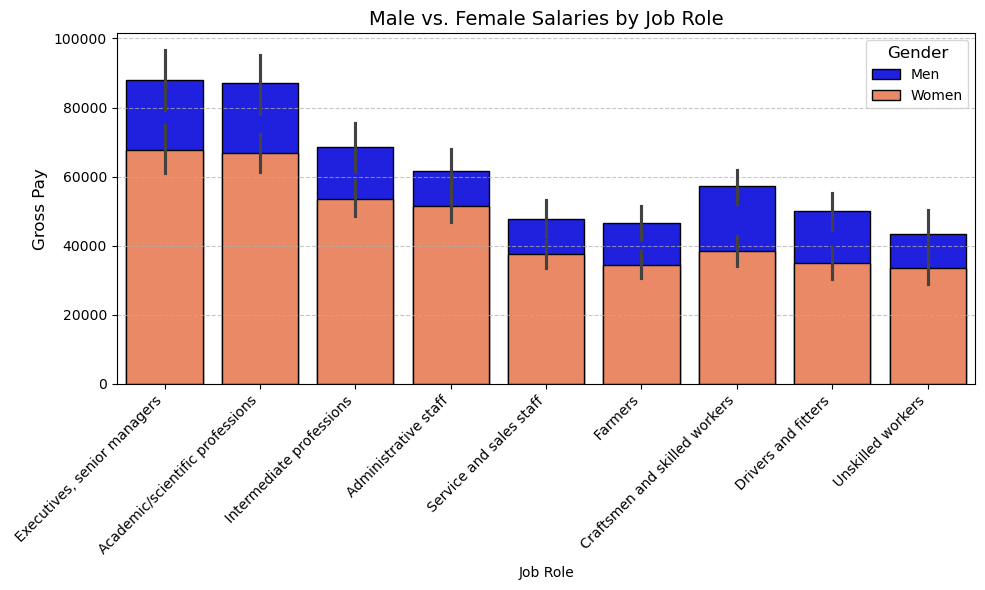
\includegraphics[width=\textwidth]{Figures/Salaries_by_Job_Role.png}
    \captionsetup{font=tiny,labelfont={color=black},justification=raggedright,singlelinecheck=off}
    \caption{Gender Pay Gap by Job Role}
    \label{fig:pay_gap_roles}
\end{figure}
  \begin{itemize}
    \item Craftsmen and skilled workers (34.59\%)
    \item Academic/Scientific Professions(22.49\%)
\end{itemize} 
\end{center}
\end{frame}


\begin{frame}
\frametitle{Relative Gender Pay Gap by Job Role}
\begin{center}
\begin{figure}[H]
    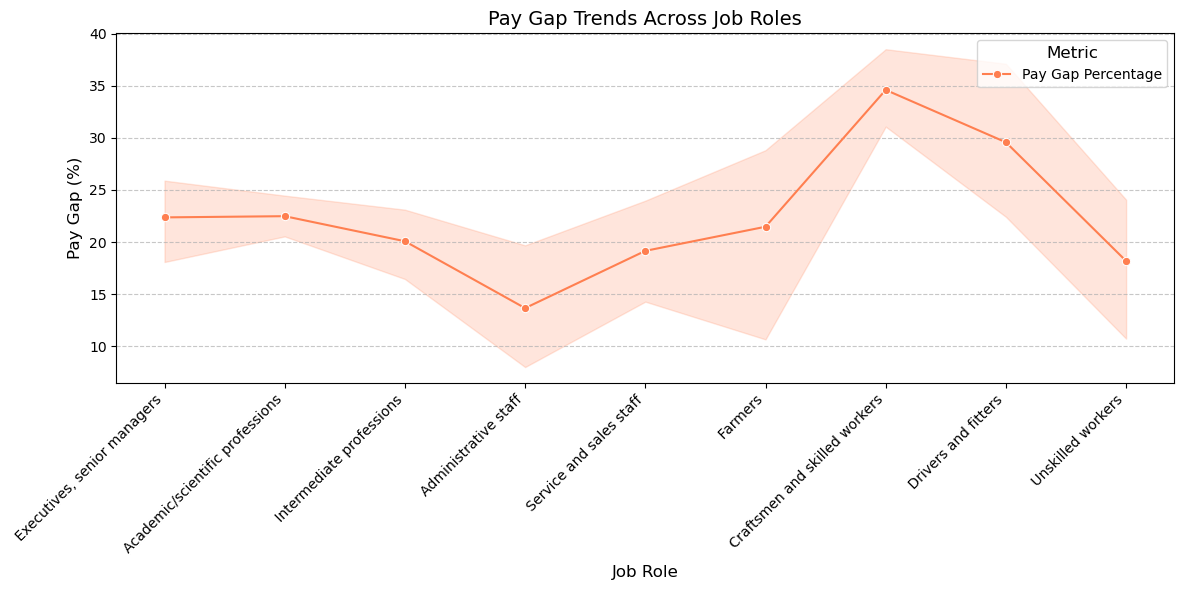
\includegraphics[width=\textwidth]{Figures/Pay_Gap_Trends_by_Job_Role.png}
    \captionsetup{font=tiny,labelfont={color=black},justification=raggedright,singlelinecheck=off}
    \caption{Relative Gender Pay Gap by Job Role}
    \label{fig:relative_gap_roles}
\end{figure}
\end{center}
\end{frame}



\begin{frame}
\frametitle{Gender Pay Gap by Job Role: Results}
\begin{center}
  \begin{itemize}
    \item Job roles with high variation aggregates very diverse specific job roles across
various industries
    \item Executives and senior manager: often male-dominated and associated with traditional gender norms.
    \item Administrative staff: often more standardized pay structures (set salary scales, fixed hourly wages)
    \item Less occupational segregation compared to other categories
    \item Administrative positions may have fewer hierarchical levels
    \item Not control over full-time versus part-time employment
\end{itemize} 
\end{center}
\end{frame}


\begin{frame}
\frametitle{Trend of Gender Pay Gap over Time}
\begin{center}
\begin{figure}[H]
    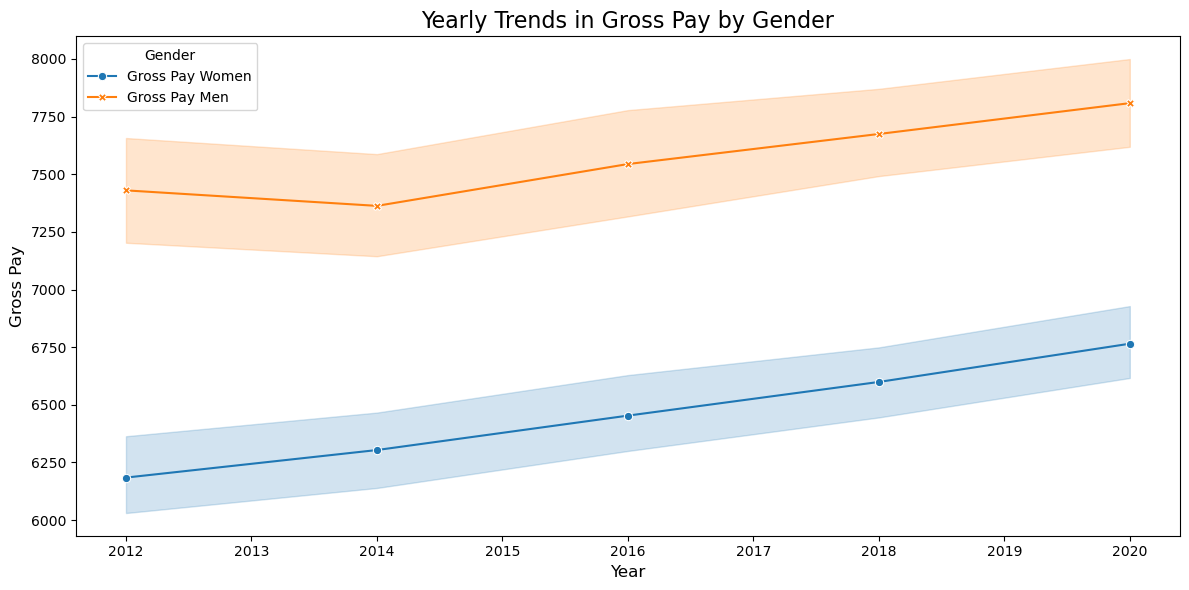
\includegraphics[width=\textwidth]{Figures/Trends_Gross_Pay_Gender.png}
    \captionsetup{font=tiny,labelfont={color=black},justification=raggedright,singlelinecheck=off}
    \caption{Trends in Gross Pay by Gender over Years}
    \label{fig:gross_trend}
\end{figure}
\end{center}
\end{frame}

\begin{frame}
\frametitle{Trend of Gender Pay Gap over Time by Job Role}
\begin{center}
\begin{figure}[H]
    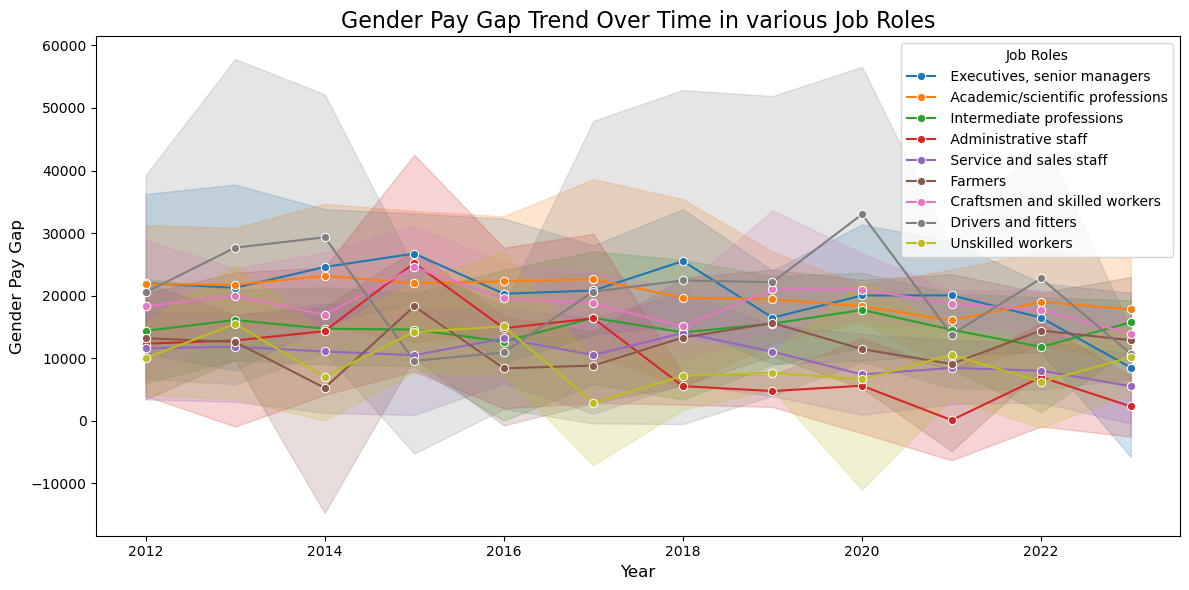
\includegraphics[width=\textwidth]{Figures/Gap_over_Time_Roles.png}
    \captionsetup{font=tiny,labelfont={color=black},justification=raggedright,singlelinecheck=off}
    \caption{Trends in Gender Pay Gap by Job Roles over Years}
    \label{fig:roles_trend}
\end{figure}
\end{center}
\end{frame}


\begin{frame}
\frametitle{Gender Pay Gap by Job Role: Results}
\begin{center}
  \begin{itemize}
    \item Job roles with high variation aggregates very diverse specific job roles across
various industries
    \item Upward trend in wages for both men and women
    \item Consistently higher wages for men compared to women
    \item Gradual narrowing of the pay gap
    \item Overall trend remains consistent across all job roles
    \item None of the job roles stands out as experiencing a disproportionately large or small reduction in the gap progress toward wage equality is
    \item Generally occurring at a similar pace across the labor market.
\end{itemize} 
\end{center}
\end{frame}


\begin{frame}
\frametitle{Severity of Gender Pay Gap by Job Role and Work Type}
\begin{center}
\begin{figure}[H]
    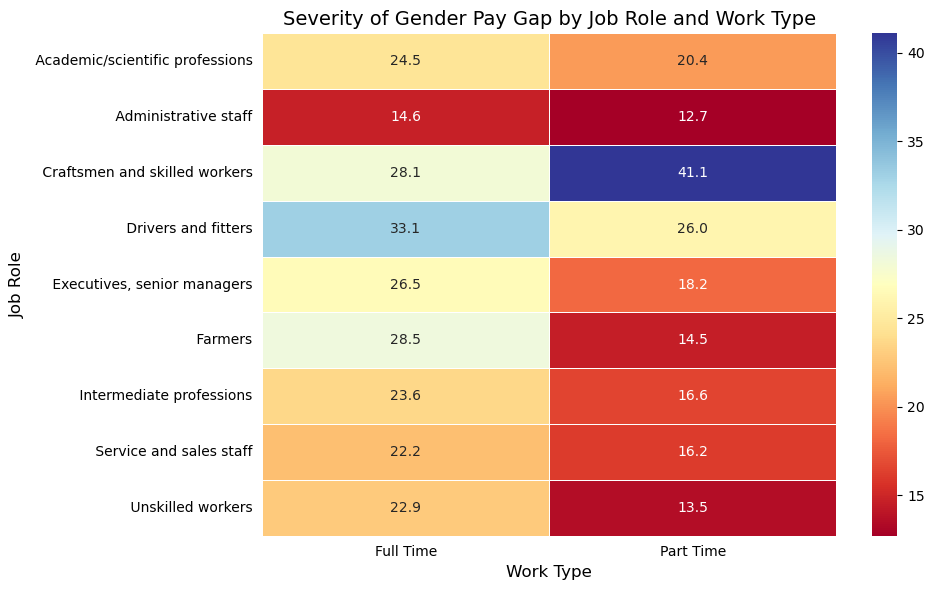
\includegraphics[width=\textwidth]{Figures/Severity_of_Pay_Gap_by_Role_and_Work_Type.png}
    \captionsetup{font=tiny,labelfont={color=black},justification=raggedright,singlelinecheck=off}
    \caption{Relative Gender Pay Gap by Job Role and Work Type}
    \label{fig:heatmap}
\end{figure}
\end{center}
\end{frame}

\begin{frame}
\frametitle{Gender Pay Gap by Job Role: Results}
\begin{center}
  \begin{itemize}
    \item Small differences indicate standardized standardized salary scales
    \item Structural and cultural factors within group of craftsmen and skilled workers
    \item Part-time roles in skilled professions may often be lower-skilled or less senior positions
    \item Part-time workers may have limited access to bonuses or specialized training opportunities, widening the gap
\end{itemize} 
\end{center}
\end{frame}


\begin{frame}
\frametitle{Distribution of Gross Pay by Gender Across Job Roles}
\begin{center}
\begin{figure}[H]
    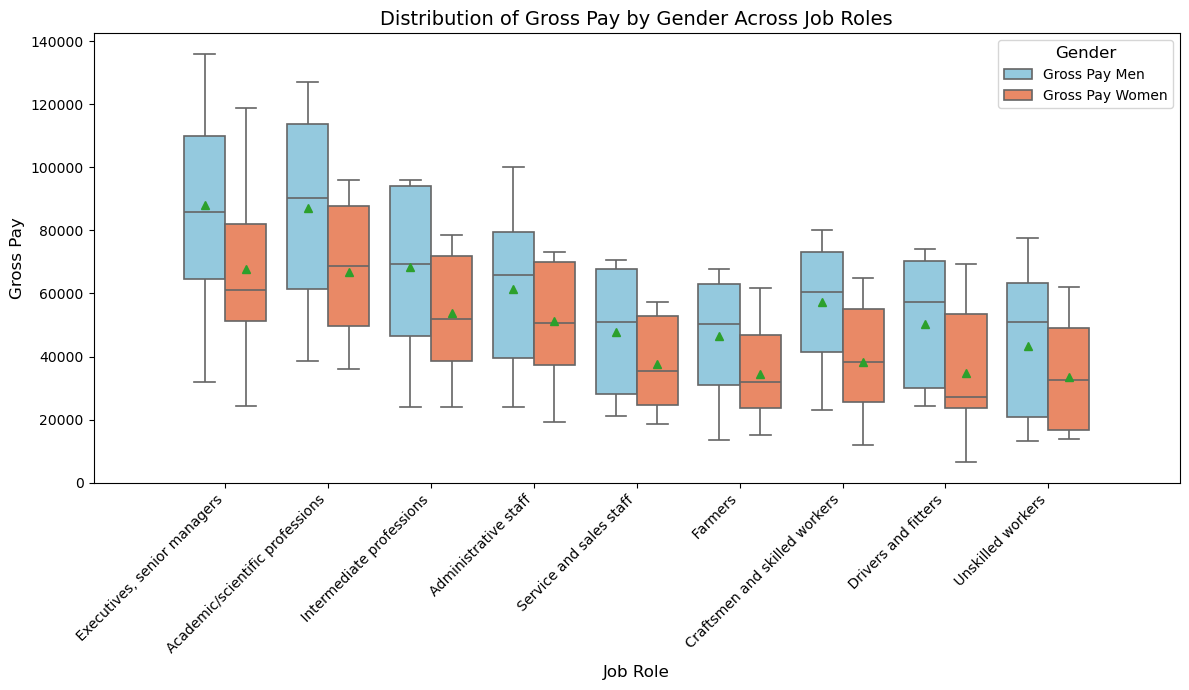
\includegraphics[width=\textwidth]{Figures/Distribution_Gross-Pay.png}
    \captionsetup{font=tiny,labelfont={color=black},justification=raggedright,singlelinecheck=off}
    \caption{Distribution of Gender Pay Gap by Job Role and Work Type}
    \label{fig:distribution_gross}
\end{figure}
\end{center}
\end{frame}


\begin{frame}
\frametitle{Distribution of Gross Pay by Gender Across Job Roles: Results}
\begin{center}
  \begin{itemize}
    \item Largest variability between men and women in Executives and senior managers
    \item Men are more likely to occupy higher-paying senior positions and more variable roles
within executive levels.
    \item Less variability in pay among female executives and senior managers
    \item Suggests a broader spread of salaries at the extremes within the female group.
    \item  ”Glass ceiling” effect
\end{itemize} 
\end{center}
\end{frame}


\subsection{Gender Pay Gap in Switzerland by Gross Regions}

\begin{frame}
\frametitle{Gross Gender Pay Gap over Time Across Gross Regions in Switzerland}
\begin{center}
\begin{figure}[H]
    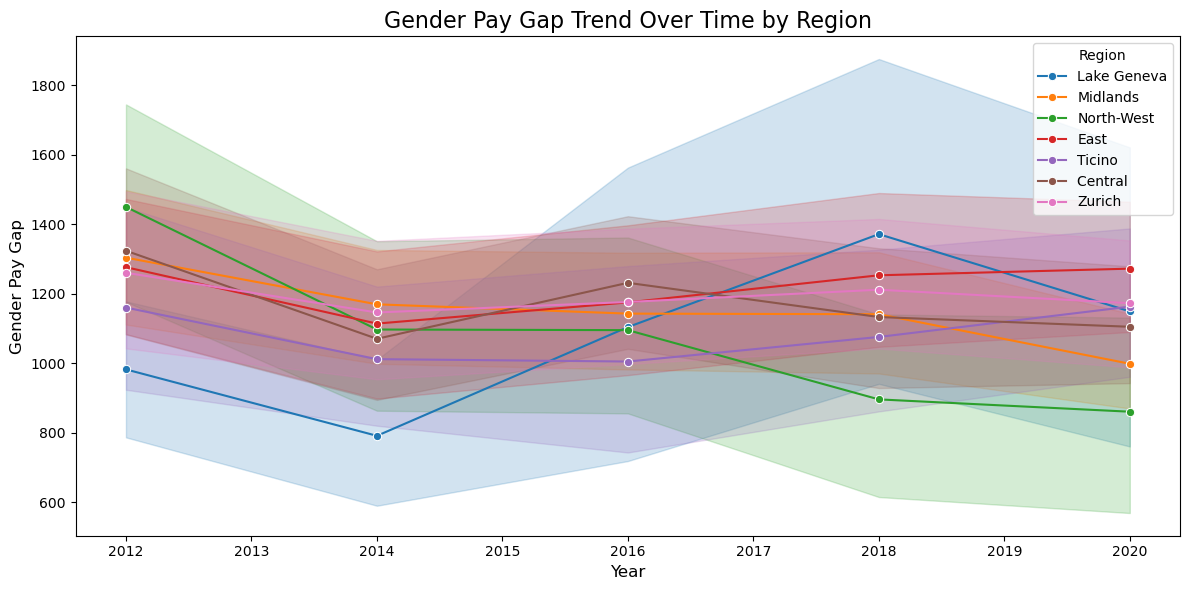
\includegraphics[width=\textwidth]{Figures/Pay_Gap_Over_Time_Region.png}
    \captionsetup{font=tiny,labelfont={color=black},justification=raggedright,singlelinecheck=off}
    \caption{Gross Gender Pay Gap over Time Across Gross Regions in Switzerland}
    \label{fig:trend_regions}
\end{figure}
\end{center}
\end{frame}

\begin{frame}
\frametitle{Gross Gender Pay Gap over Time Across Gross Regions in Switzerland: Results}
\begin{center}
  \begin{itemize}
    \item Downward trend in the gender pay gap across Switzerland’s gross regions over time
    \begin{itemize}
    \item Largest decline in the gender pay gap is found in the North-West region (Basel & Aargau)
    \item High concentration of multinational corporations in the pharmaceutical, finance and technology sectors.
    \item Region may have seen a greater number of women entering high-paying sectors and leadership roles, contributing to the narrowing of the pay gap
    \end{itemize} 
\end{itemize} 
\end{center}
\end{frame}


\begin{frame}
\frametitle{Absolute Gender Pay Gap by Region}
\begin{center}
\begin{figure}[H]
    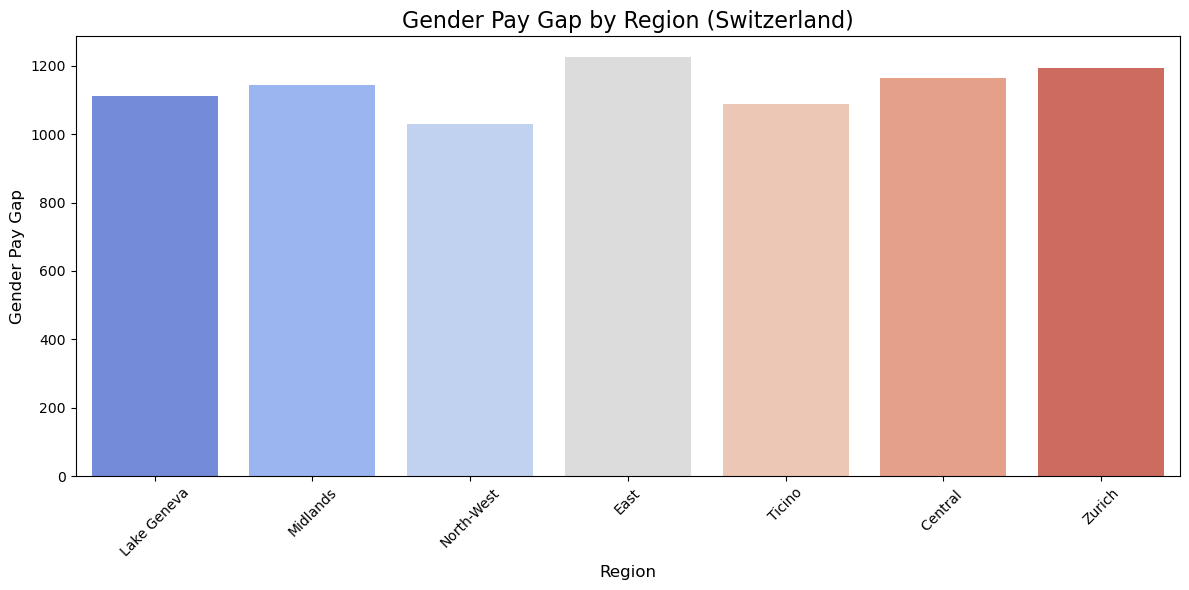
\includegraphics[width=\textwidth]{Figures/Gross_Pay_Gap_Region.png}
    \captionsetup{font=tiny,labelfont={color=black},justification=raggedright,singlelinecheck=off}
    \caption{Gender Pay Gap by Region}
    \label{fig:gap_regions}
\end{figure}
\end{center}
\end{frame}

\begin{frame}
\frametitle{Gross Gender Pay Ratio by Region}
\begin{center}
\begin{figure}[H]
    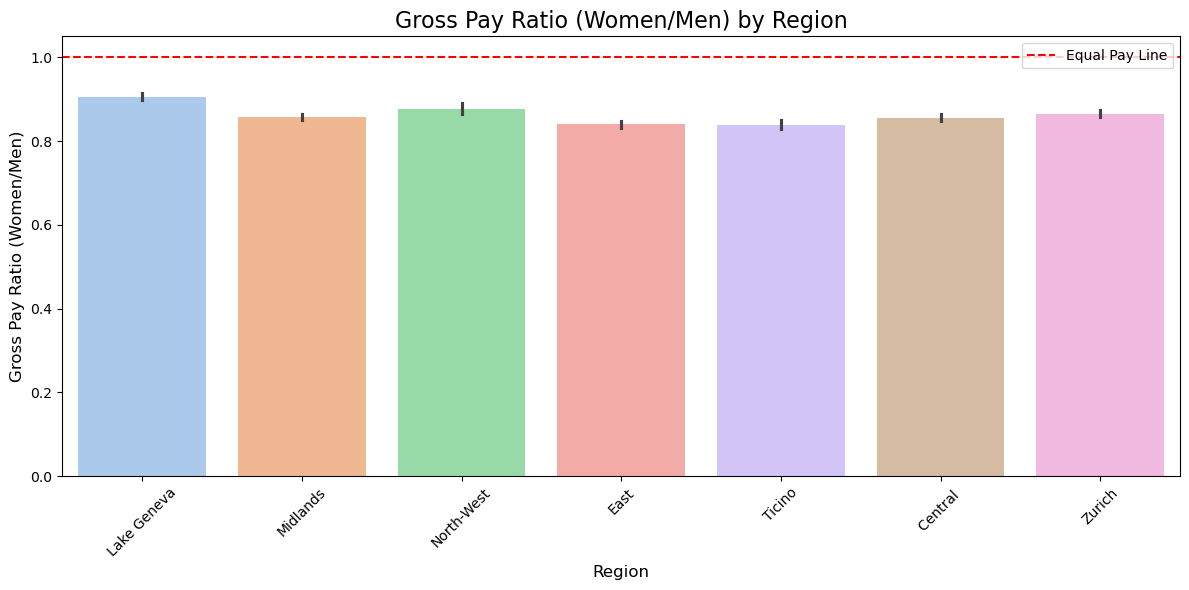
\includegraphics[width=\textwidth]{Figures/Gross_Ratio_Region.png}
    \captionsetup{font=tiny,labelfont={color=black},justification=raggedright,singlelinecheck=off}
    \caption{Ratio of Gross Wages by Region}
    \label{fig:ratio_region}
\end{figure}
\end{center}
\end{frame}

\begin{frame}
\frametitle{Gender Pay Gap by Region}
\begin{center}
  \begin{itemize}
    \item Wage disparities between men and women are reltively consistent nationwide, no region displaying significantly higher or lower gaps
    \item Suggests that the gender pay gap is a pervasive issue across Switzerland
    \item Gender Pay Ratio across regions falls consistently between 0.8 and 0.9
\begin{itemize}
    \item Women earn approximately 80-90% of what men earn
\end{itemize} 
\end{itemize} 
\end{center}
\end{frame}


\section{Conclusion}
\begin{frame}
\frametitle{Conclusion}
\begin{itemize}
  \item Confirms the existence of a persistent gender pay gap in Switzerland
  \item Significant differences are observed across industries
  \item Over the observed time frame, the gender pay gap has shown a gradual decrease
  \item Regional differences in the pay gap were identified, but the variations in absolute terms were found to be relatively minor
  \item Regional disparities are less pronounced than those seen across industries.
  \end{itemize}  
\end{frame}








\end{document}